% !TeX program = xelatex
\documentclass[a4paper,10pt]{article}

% ============================================================================
% សន្លឹកកិច្ចការសិស្សបំពេញចន្លោះ ស-ខ្មៅ និងប្លង់ក្ដារខៀន/ចម្លើយគ្រូ (គ្មាន LCD / គ្មានកន្ត្រៃ)
% មេរៀនទី៤ (៤)៖ ល្បឿនមធ្យម — ត្រូវគ្នា ១០០% នឹង LS_Plan_MEAS44.tex
% ============================================================================
\usepackage[a4paper, left=1.0cm, right=1.0cm, top=0.75cm, bottom=1.00cm, footskip=0.52cm]{geometry}
\usepackage{amsmath}
\usepackage{unicode-math}
\usepackage{fontspec}
\usepackage{array, colortbl}
\usepackage[table]{xcolor}
\usepackage{enumitem}
\usepackage{pifont}
\usepackage{fancyhdr}
\usepackage{lastpage}
\usepackage{tikz}
\usepackage[most]{tcolorbox}
\usetikzlibrary{calc, arrows.meta, decorations.pathreplacing, positioning, babel}

\makeatletter
\let\@expl@@@mark@update@singlecol@structures@@\relax
\makeatother

\providecommand{\NGSFindFonts}{%
  \IfFileExists{C:/Windows/Fonts/cambria.ttc}{%
    \def\NGSSysPath{C:/Windows/Fonts/}%
    \def\NGSUserPath{C:/Users/KIT/AppData/Local/Microsoft/Windows/Fonts/}%
  }{%
    \IfFileExists{./fonts/KhmerOSsiemreap.ttf}{\def\NGSSysPath{./fonts/}\def\NGSUserPath{./fonts/}}{%
    \IfFileExists{../fonts/KhmerOSsiemreap.ttf}{\def\NGSSysPath{../fonts/}\def\NGSUserPath{../fonts/}}{%
    \IfFileExists{../../fonts/KhmerOSsiemreap.ttf}{\def\NGSSysPath{../../fonts/}\def\NGSUserPath{../../fonts/}}{%
    \IfFileExists{../../../fonts/KhmerOSsiemreap.ttf}{\def\NGSSysPath{../../../fonts/}\def\NGSUserPath{../../../fonts/}}{%
    \IfFileExists{../../../../fonts/KhmerOSsiemreap.ttf}{\def\NGSSysPath{../../../../fonts/}\def\NGSUserPath{../../../../fonts/}}{%
    \IfFileExists{../../../../../fonts/KhmerOSsiemreap.ttf}{\def\NGSSysPath{../../../../../fonts/}\def\NGSUserPath{../../../../../fonts/}}{%
    \IfFileExists{../../../../../../fonts/KhmerOSsiemreap.ttf}{\def\NGSSysPath{../../../../../../fonts/}\def\NGSUserPath{../../../../../../fonts/}}{%
      \def\NGSSysPath{../../../../../../../fonts/}\def\NGSUserPath{../../../../../../../fonts/}%
    }}}}}}}%
  }%
}
\NGSFindFonts

\setmathfont[Path={\NGSSysPath}, FontIndex=1, Scale=1.02]{cambria.ttc}
\defaultfontfeatures{Ligatures=TeX}

\setmainfont[
  Path={\NGSUserPath}, Extension=.ttf, Script=Khmer,
  BoldFont={KhmerOSsiemreap}, BoldFeatures={FakeBold=1.8},
  ItalicFont={KhmerOSsiemreap}, ItalicFeatures={FakeSlant=0.25},
  BoldItalicFont={KhmerOSsiemreap}, BoldItalicFeatures={FakeBold=1.8, FakeSlant=0.25}
]{KhmerOSsiemreap}

\newfontfamily\muol[Path={\NGSUserPath}, Extension=.ttf, Script=Khmer]{KhmerOSmuollight}
\newfontfamily\TimesEn[Path={\NGSSysPath}, Extension=.ttf, BoldFont={timesbd}, ItalicFont={timesi}, BoldItalicFont={timesbi}]{times}
\newfontfamily\CalibriFont[Path={\NGSSysPath}, Extension=.ttf]{calibri}

\XeTeXlinebreaklocale "km"
\XeTeXlinebreakskip = 0pt plus 1pt minus 0.1pt

\definecolor{panelgray}{gray}{0.94}
\definecolor{headgray}{gray}{0.85}

\pagestyle{fancy}
\fancyhf{}
\renewcommand{\headrulewidth}{0pt}
\fancyfoot[L]{\fontsize{7.4pt}{9.5pt}\selectfont អនុវិទ្យាល័យព្រះក្រសាំង \en{|} គ្រូ៖ ហុក ប៊ុនថែន \en{|} មេរៀនទី៤ (៤) ល្បឿនមធ្យម \en{|} ថ្ងៃព្រហស្បតិ៍ ទី៣ ខែធ្នូ ឆ្នាំ២០២៦}
\fancyfoot[R]{\fontsize{7.8pt}{10pt}\selectfont ទំព័រ \en{\thepage\ / \pageref{LastPage}}}

\setlength{\parindent}{0pt}
\setlength{\parskip}{0pt}
\setlength{\tabcolsep}{4pt}

\newcommand{\en}[1]{{\TimesEn #1}}
\newcommand{\enbf}[1]{{\TimesEn\bfseries #1}}
\newcommand{\unit}[1]{\,\text{\en{#1}}}
\newcommand{\riel}{\,\text{៛}}
\newcommand{\cnum}[1]{\mbox{\fontsize{10pt}{12pt}\selectfont\ding{\numexpr181+#1\relax}}}
\newcommand{\chkbox}{\tikz[baseline=-0.15ex]\draw[black, line width=0.85pt, fill=white] (0,0) rectangle (0.24cm,0.24cm);}
\newcommand{\ansbox}[1][1.75cm]{\,\tikz[baseline=-0.65ex]\draw[black, line width=0.65pt, fill=white] (0,0) rectangle (#1, 0.42cm);\,}
\newcommand{\dotline}[1][2.2cm]{\makebox[#1]{\dotfill}}

\newcommand{\pagebanner}[2]{%
  \begin{tcolorbox}[
    enhanced, sharp corners, colback=headgray, colframe=black,
    boxrule=1.05pt, boxsep=1pt, top=2.5pt, bottom=2.5pt, left=6pt, right=6pt,
    after skip=3.5pt
  ]
    {\muol\fontsize{9.0pt}{13.2pt}\selectfont #1}\hfill{\fontsize{8.0pt}{11.2pt}\selectfont\textbf{#2}}
  \end{tcolorbox}%
}

\newcommand{\secstrip}[2]{%
  \vspace{3pt}%
  \begin{tcolorbox}[
    enhanced, sharp corners, colback=panelgray, colframe=black,
    boxrule=0.8pt, boxsep=0.8pt, top=2pt, bottom=2pt, left=5pt, right=5pt,
    after skip=3pt
  ]
    {\muol\fontsize{8.5pt}{12.2pt}\selectfont #1}\hfill{\fontsize{7.8pt}{10.8pt}\selectfont\textit{#2}}
  \end{tcolorbox}%
}

\newcolumntype{L}[1]{>{\raggedright\arraybackslash}p{#1}}
\newcolumntype{C}[1]{>{\centering\arraybackslash}p{#1}}

\begin{document}
\fontsize{9.5pt}{14.5pt}\selectfont

% ============================================================================
% ទំព័រទី ១៖ សន្លឹកកិច្ចការសិស្ស (ផ្នែកមុខ៖ E1 -> E2 -> E3)
% ============================================================================
\pagebanner{សន្លឹកកិច្ចការសិស្ស \enbf{(}៤\enbf{.}៤ ល្បឿនមធ្យម\enbf{)} \enbf{--} ផ្នែកមុខ}{ថ្នាក់ទី៨ \en{|} សៀវភៅគោល ទំ.៤៨--៤៩}

\begin{tcolorbox}[
  enhanced, sharp corners, colback=white, colframe=black,
  boxrule=0.8pt, boxsep=1.5pt, top=3.5pt, bottom=3.5pt, left=5pt, right=5pt,
  after skip=4pt
]
  \fontsize{9.0pt}{13.0pt}\selectfont
  \textbf{ឈ្មោះសិស្ស៖} \dotline[4.3cm] \quad
  \textbf{សមាជិកក្រុម៖} \dotline[4.3cm] \quad
  \textbf{ថ្នាក់ទី៖} ៨\dotline[0.9cm] \quad
  \textbf{ក្រុមទី៖} \dotline[1.0cm]
\end{tcolorbox}

% --- E1 Engage ---
\secstrip{ផ្នែកទី ១ \enbf{(E1 - Engage)} ៖ បេសកកម្មអន្ទាក់ម៉ោងនិងនាទីលើល្បឿនម៉ូតូ}{រយៈពេល ៣ នាទី (គូស \ding{51} ក្នុង \chkbox)}

\begin{tcolorbox}[
  enhanced, sharp corners, colback=white, colframe=black,
  boxrule=0.8pt, boxsep=2pt, top=3.5pt, bottom=3.5pt, left=6pt, right=6pt
]
  ទោចក្រយានយន្តមួយរត់បានចម្ងាយ $108\unit{km}$ ក្នុងរយៈពេល $2\unit{h}\,15\unit{mn}$ ។\\[2pt]
  $\bullet$ \textbf{តើសិស្សរូបណាបំប្លែងរយៈពេល និងគណនាល្បឿនមធ្យមបានត្រឹមត្រូវ?} \quad
  \chkbox\ \textbf{សិស្ស ក៖} $2.15\unit{h} \implies 50.2\unit{km/h}$ \qquad
  \chkbox\ \textbf{សិស្ស ខ៖} $2.25\unit{h} \implies 48\unit{km/h}$\\[2pt]
  $\bullet$ \textbf{ហេតុផលខ្លី៖} ក្នុង $1\unit{h}$ មាន $60\unit{mn}$ ដូចនេះ $15\unit{mn} = \dfrac{15}{60}\unit{h} =$ \dotline[2.4cm] $\unit{h}$ ។
\end{tcolorbox}

\vfill

% --- E2 Explore ---
\secstrip{ផ្នែកទី ២ \enbf{(E2 - Explore)} ៖ ឧទាហរណ៍ទី ១ និងស្ពានបំប្លែងខ្នាតល្បឿន (ទំ.៤៨--៤៩)}{រយៈពេល ១១ នាទី}

\textbf{សកម្មភាព ១ (\en{E2-A} — ៦ នាទី)៖ ខ្នាតល្បឿន (ទំ.៤៨) និងការគណនាឧទាហរណ៍ទី ១ (ទំ.៤៩)}

\begin{tcolorbox}[
  enhanced, sharp corners, colback=white, colframe=black,
  boxrule=0.8pt, boxsep=2pt, top=3.5pt, bottom=3.5pt, left=6pt, right=6pt
]
  $\bullet$ \textbf{ខ្នាតល្បឿន (ទំ.៤៨)៖} ម៉ូតូ $40\unit{km/h}$, រថយន្ត $80\unit{km/h}$, យន្តហោះ $800\unit{km/h}$; រូបវិទ្យា៖ សំឡេង $343\unit{m/s}$, ខ្យល់បក់មធ្យម $6\unit{m/s}$ ។\\[3pt]
  $\bullet$ \textbf{ឧទាហរណ៍ទី ១ (ទំ.៤៩ — ចម្ងាយចរ $d = 108\unit{km}$, រយៈពេល $t = 2\unit{h}\,15\unit{mn}$)៖}\\[2.5pt]
  \hspace*{0.3cm}១) បំប្លែងរយៈពេលជាប្រភាគម៉ោង៖ $t = 2\unit{h}\,15\unit{mn} = \left(2 + \dfrac{15}{60}\right)\unit{h} = \left(2 + \dfrac{1}{\dotline[0.8cm]}\right)\unit{h} =$ \ansbox[1.6cm] $\unit{h}$\\[3pt]
  \hspace*{0.3cm}២) គណនាល្បឿនមធ្យម៖ $v = 108 \div \dfrac{9}{4} = 108 \times \dfrac{4}{\dotline[0.8cm]} =$ \ansbox[2.0cm] $\unit{km/h}$
\end{tcolorbox}

\vspace{3pt}
\textbf{សកម្មភាព ២ (\en{E2-B} — ៥ នាទី)៖ បង្កើតស្ពានបំប្លែងខ្នាតល្បឿនពី $\unit{m/s}$ ទៅ $\unit{km/h}$}

\begin{tcolorbox}[
  enhanced, sharp corners, colback=white, colframe=black,
  boxrule=0.8pt, boxsep=2pt, top=3.5pt, bottom=3.5pt, left=6pt, right=6pt
]
  $\bullet$ បើវត្ថុរត់បាន $1\unit{m}$ ក្នុង $1\unit{s}$ នោះក្នុង $1\unit{h} = 3\,600\unit{s}$ វារត់បាន $3\,600\unit{m} =$ \dotline[1.6cm] $\unit{km} \implies 1\unit{m/s} =$ \ansbox[1.6cm] $\unit{km/h}$ ។\\[2.5pt]
  $\bullet$ \textbf{អនុវត្ត៖} ល្បឿនខ្យល់បក់មធ្យម $6\unit{m/s} = 6 \times 3.6 =$ \dotline[1.8cm] $\unit{km/h}$; ចុះ $72\unit{km/h} = 72 \div 3.6 =$ \dotline[1.6cm] $\unit{m/s}$ ។
\end{tcolorbox}

\vfill

% --- E3 Explain ---
\secstrip{ផ្នែកទី ៣ \enbf{(E3 - Explain)} ៖ រូបមន្តល្បឿនមធ្យម និងធនាគារហេតុផល \enbf{B\&W}}{រយៈពេល ៦ នាទី}

\begin{tcolorbox}[
  enhanced, sharp corners, colback=white, colframe=black,
  boxrule=0.85pt, boxsep=2pt, top=3.5pt, bottom=3.5pt, left=6pt, right=6pt
]
  ១) \textbf{ល្បឿនមធ្យម៖} $v = \dfrac{d}{\dotline[0.8cm]}$ \qquad
  ២) \textbf{ចម្ងាយចរ៖} $d = v \times \dotline[0.8cm]$ \qquad
  ៣) \textbf{រយៈពេល៖} $t = \dfrac{d}{\dotline[0.8cm]}$ \qquad
  ៤) $1\unit{m/s} =$ \dotline[1.2cm] $\unit{km/h}$\\[4pt]
  \tikz\draw[black, dashed, line width=0.5pt] (0,0) -- (18.4cm,0);\\[3pt]
  \fontsize{8.8pt}{12.8pt}\selectfont
  \textbf{ធនាគារហេតុផល (\en{Warrant Bank})៖} \quad
  \cnum{1} \textbf{ពេលគោល $60$៖} $t(\unit{h}) = h + \frac{\text{mn}}{60} + \frac{\text{s}}{3\,600}$ \quad
  \cnum{2} \textbf{ស្ពានល្បឿន៖} $\unit{m/s} \xrightarrow{\times 3.6} \unit{km/h}$ និង $\unit{km/h} \xrightarrow{\div 3.6} \unit{m/s}$\\
  \cnum{3} \textbf{រូបមន្ត៖} $v = \frac{d}{t}, \ d = vt, \ t = \frac{d}{v}$ \quad
  \cnum{4} \textbf{ឯកភាពខ្នាត៖} $(v\text{ ជា }\unit{m/s}, t\text{ ជា }\unit{s} \implies d\text{ ជា }\unit{m})$ ឬ $(v\text{ ជា }\unit{km/h}, t\text{ ជា }\unit{h} \implies d\text{ ជា }\unit{km})$
\end{tcolorbox}

% ============================================================================
% ទំព័រទី ២៖ សន្លឹកកិច្ចការសិស្ស (ផ្នែកខាងខ្នង៖ E4 -> E5 -> កិច្ចការផ្ទះ)
% ============================================================================
\clearpage
\pagebanner{សន្លឹកកិច្ចការសិស្ស \enbf{(}៤\enbf{.}៤ ល្បឿនមធ្យម\enbf{)} \enbf{--} ផ្នែកខាងខ្នង}{ថ្នាក់ទី៨ \en{|} សៀវភៅគោល ទំ.៤៩--៥០}

% --- E4 Elaborate ---
\secstrip{ផ្នែកទី ៤ \enbf{(E4 - Elaborate)} ៖ លំហាត់គំរូ — សំឡេងកាំភ្លើងធំពីទីក្រុង \enbf{A} ទៅទីក្រុង \enbf{B} (ទំ.៤៩)}{រយៈពេល ១០ នាទី}

\begin{tcolorbox}[
  enhanced, sharp corners, colback=white, colframe=black,
  boxrule=0.8pt, boxsep=2pt, top=3.5pt, bottom=3.5pt, left=6pt, right=6pt
]
  គេបាញ់កាំភ្លើងធំដើម្បីប្រារព្ធពិធីបុណ្យនៅទីក្រុង $A$ នៅម៉ោង $0$ កណ្ដាលយប់ ។ បន្ទាប់ពីការបាញ់ $1\unit{mn}$ ក្រោយមកទើបប្រជាជននៅទីក្រុង $B$ បានឮសំឡេងបាញ់ ។ រកចម្ងាយរវាងទីក្រុង $A$ និងទីក្រុង $B$ ដោយដឹងថាល្បឿនសំឡេង $v = 343\unit{m/s}$ ៖\\[2.5pt]
  $\bullet$ \textbf{ជំហានទី ១ (បំប្លែងរយៈពេលឱ្យត្រូវខ្នាត \cnum{4})៖} $t = 1\unit{mn} =$ \dotline[1.6cm] $\unit{s}$\\[3pt]
  $\bullet$ \textbf{ជំហានទី ២ (គណនាចម្ងាយជាម៉ែត្រ និងគីឡូម៉ែត្រ \cnum{3})៖} $x = v \times t = 343\unit{m/s} \times$ \dotline[1.4cm] $\unit{s} =$ \dotline[2.0cm] $\unit{m} =$ \ansbox[2.0cm] $\unit{km}$\\[2pt]
  \fontsize{8.7pt}{12.5pt}\selectfont
  \textbf{ឆ្លុះបញ្ចាំង (\en{EIA Looking-Back})៖} ព្រោះ $1\unit{km} = 1\,000\unit{m}$ ដូច្នេះ $20\,580\unit{m} \div 1\,000 =$ \dotline[1.6cm] $\unit{km}$ (កុំច្រឡំដាក់ក្បៀសជា $2.06\unit{km}$!) ។
\end{tcolorbox}

\vfill

% --- E5 Evaluate ---
\secstrip{ផ្នែកទី ៥ \enbf{(E5 - Evaluate)} ៖ លំហាត់ប្រតិបត្តិពពករសាត់ (ទំ.៤៩) សំណួរវិនិច្ឆ័យ \enbf{A--D} និងសំបុត្រចេញ}{រយៈពេល ១០ នាទី}

\begin{tcolorbox}[
  enhanced, sharp corners, colback=white, colframe=black,
  boxrule=0.8pt, boxsep=2pt, top=3.5pt, bottom=3.5pt, left=6pt, right=6pt
]
  \textbf{១) ប្រតិបត្តិ (ទំ.៤៩)៖} ពពកមួយផ្ទាំងធំកំពុងរសាត់ពីសមុទ្រនៃខេត្តព្រះសីហនុមកកាន់រាជធានីភ្នំពេញ ដែលមានចម្ងាយប្រមាណ $d = 230\unit{km}$ ហើយខ្យល់មានល្បឿន $v = 6\unit{m/s}$ ។ តើរយៈពេលប៉ុន្មានម៉ោងទៀតទើបនៅរាជធានីភ្នំពេញសង្ឃឹមថានឹងមានភ្លៀង?\\[3pt]
  $\bullet$ បំប្លែងល្បឿនខ្យល់ជា $\unit{km/h}$ (\cnum{2})៖ $v = 6\unit{m/s} = 6 \times 3.6 =$ \dotline[1.8cm] $\unit{km/h}$\\[3pt]
  $\bullet$ គណនារយៈពេល (\cnum{3})៖ $t = \dfrac{d}{v} = \dfrac{230}{\dotline[1.6cm]} \approx$ \ansbox[2.2cm] $\unit{h}$ ($\approx 10\unit{h}\,39\unit{mn}$)\\[3pt]
  \textbf{២) បិទបេសកកម្ម \en{E1}៖} សិស្ស \dotline[0.9cm] ត្រឹមត្រូវ ព្រោះ $2\unit{h}\,15\unit{mn} = 2.25\unit{h}$ នាំឱ្យល្បឿនមធ្យមស្មើ \dotline[1.5cm] $\unit{km/h}$ ។
\end{tcolorbox}

\vspace{3.5pt}

\begin{tcolorbox}[
  enhanced, sharp corners, colback=white, colframe=black,
  boxrule=0.8pt, boxsep=2pt, top=3.5pt, bottom=3.5pt, left=6pt, right=6pt
]
  \textbf{៣) សំណួរវិនិច្ឆ័យ \en{A--D} (រថយន្តមួយរត់បានចម្ងាយ $90\unit{km}$ ក្នុងរយៈពេល $1\unit{h}\,30\unit{mn}$ តើល្បឿនមធ្យមស្មើប៉ុន្មាន $\unit{km/h}$? — លើកម្រាមដៃ ១--៤)៖}\\[2.5pt]
  \textbf{\en{A.}} $69.2\unit{km/h}$ \qquad
  \textbf{\en{B.}} $60\unit{km/h}$ \qquad
  \textbf{\en{C.}} $135\unit{km/h}$ \qquad
  \textbf{\en{D.}} $1\unit{km/h}$\\[3.5pt]
  \tikz\draw[black, dashed, line width=0.5pt] (0,0) -- (18.4cm,0);\\[3pt]
  \textbf{៤) សំបុត្រចេញ ៦០ វិនាទី៖} បំប្លែងល្បឿន $v = 10\unit{m/s} =$ \dotline[1.6cm] $\unit{km/h}$;
  បើរត់ក្នុងរយៈពេល $t = 30\unit{mn} = 0.5\unit{h}$ បានចម្ងាយ $d =$ \dotline[1.6cm] $\unit{km}$ ។
\end{tcolorbox}

\vfill

% --- Homework ---
\begin{tcolorbox}[
  enhanced, sharp corners, colback=panelgray, colframe=black,
  boxrule=0.95pt, boxsep=2pt, top=3.5pt, bottom=3.5pt, left=6pt, right=6pt
]
  {\muol\fontsize{9.0pt}{13.0pt}\selectfont កិច្ចការផ្ទះបញ្ចប់មេរៀនទី៤ \enbf{(}សៀវភៅគោល ទំ.៥០ លេខ ៧, ៨ និង ៩\enbf{)}}\\[2.5pt]
  \fontsize{8.7pt}{12.8pt}\selectfont
  $\bullet$ \textbf{\#7៖} នៅថ្ងៃអាទិត្យ វិបុលជិះកង់ពីក្រុងតាខ្មៅទៅទន្លេបាទីចម្ងាយ $26\unit{km}$ ក្នុងរយៈពេល $41\unit{mn}\,52\unit{s}$ ។ រកល្បឿនមធ្យមក្នុងមួយម៉ោង ។\\
  $\bullet$ \textbf{\#8៖} ផ្ទះរតនានៅចម្ងាយ $800\unit{m}$ ពីសាលារៀន ដើរដោយល្បឿនមធ្យម $5\unit{km/h}$ ។ តើរតនាត្រូវចេញពីផ្ទះនៅម៉ោងប៉ុន្មាន ដើម្បីឱ្យទៅដល់សាលារៀន $15\unit{mn}$ មុនពេលចូលរៀនម៉ោង $7\unit{h}\,00\unit{mn}$?\\
  $\bullet$ \textbf{\#9៖} នៅម៉ោង $7:00$ សុខាជិះរថភ្លើងពីបាត់ដំបងមកភ្នំពេញ ($291\unit{km}$, ល្បឿន $60\unit{km/h}$) ឯមករាជិះម៉ូតូពីភ្នំពេញទៅបាត់ដំបង (ល្បឿន $40\unit{km/h}$) ។ តើអ្នកទាំងពីរជួបគ្នានៅម៉ោងប៉ុន្មាន?
\end{tcolorbox}

% ============================================================================
% ទំព័រទី ៣៖ ទំព័រគ្រូបង្រៀន (គំរូប្លង់ក្ដារខៀន ៣ ផ្នែក + ចម្លើយផ្ទៀងផ្ទាត់រហ័ស)
% ============================================================================
\clearpage
\pagebanner{ទំព័រគ្រូបង្រៀន ៖ ប្លង់ក្ដារខៀន \enbf{(}គ្មាន \enbf{LCD)} និងចម្លើយផ្ទៀងផ្ទាត់រហ័ស}{៤.៤ ល្បឿនមធ្យម (\en{MEAS44})}

\secstrip{១. គំរូប្លង់បែងចែកក្ដារខៀន ៣ ផ្នែក សម្រាប់ថ្នាក់រៀនគ្មាន \enbf{LCD}}{សម្រាប់គ្រូប្រើដីស/ហ្វឺត}

\begin{center}
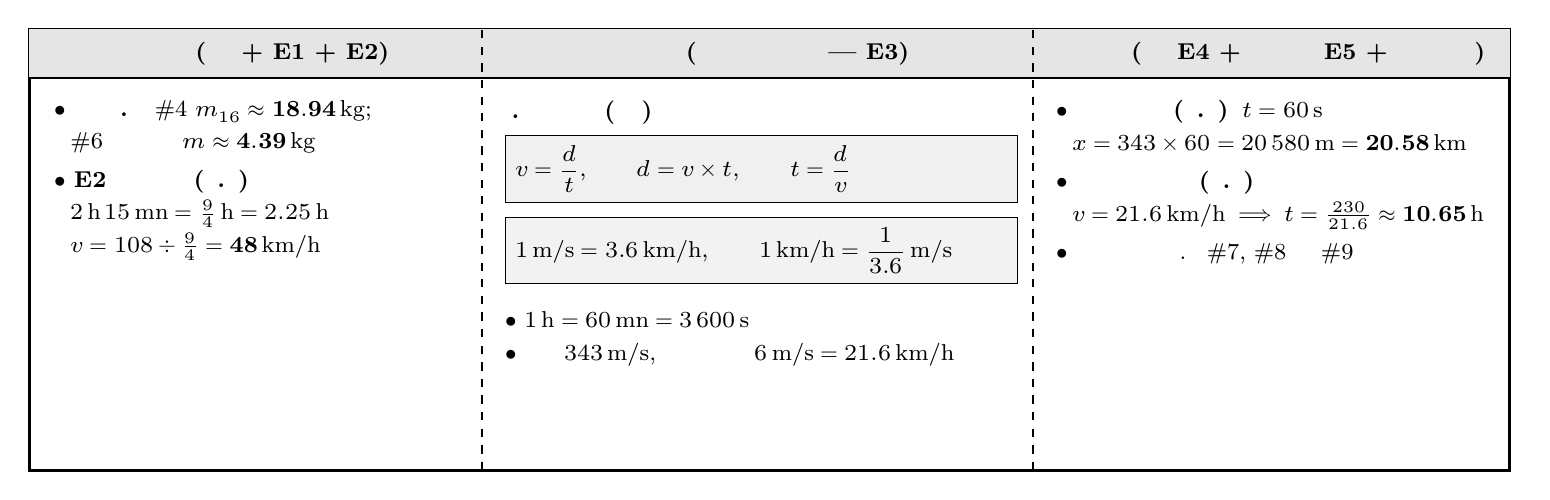
\begin{tikzpicture}[x=1cm, y=1cm, every node/.style={font=\fontsize{8.3pt}{11.8pt}\selectfont, text=black}]
  \draw[black, line width=1.1pt] (0,0) rectangle (18.8,5.60);
  \fill[gray!20] (0,4.98) rectangle (18.8,5.60);
  \draw[black, line width=0.7pt] (0,4.98) -- (18.8,4.98);
  \draw[black, dashed, line width=0.7pt] (5.75,0) -- (5.75,5.60);
  \draw[black, dashed, line width=0.7pt] (12.75,0) -- (12.75,5.60);

  \node at (2.875,5.29) {\textbf{ផ្នែកឆ្វេង (កំណែ + \en{E1} + \en{E2})}};
  \node at (9.25,5.29) {\textbf{ផ្នែកកណ្ដាល (ខ្លឹមសារគោលរក្សាទុក — \en{E3})}};
  \node at (15.775,5.29) {\textbf{ផ្នែកស្ដាំ (គំរូ \en{E4} + ប្រតិបត្តិ \en{E5} + កិច្ចការផ្ទះ)}};

  % Left
  \node[anchor=north west, text width=5.35cm] at (0.20,4.82) {%
    $\bullet$ \textbf{កំណែ ទំ.៥០៖} \#4 $m_{16} \approx \mathbf{18.94\unit{kg}}$;\\
    \hspace*{0.2cm}\#6 ខ្សែស្ពាន់ $m \approx \mathbf{4.39\unit{kg}}$\\[2pt]
    $\bullet$ \textbf{\en{E2} ឧទាហរណ៍ទី ១ (ទំ.៤៩)៖}\\
    \hspace*{0.2cm}$2\unit{h}\,15\unit{mn} = \tfrac{9}{4}\unit{h} = 2.25\unit{h}$\\
    \hspace*{0.2cm}$v = 108 \div \tfrac{9}{4} = \mathbf{48\unit{km/h}}$
  };

  % Center
  \node[anchor=north west, text width=6.65cm] at (5.92,4.82) {%
    {\muol\fontsize{8.5pt}{12pt}\selectfont ៤\enbf{.} ល្បឿនមធ្យម \enbf{(}តចប់\enbf{)}}\\[3pt]
    \tikz\node[draw=black, fill=gray!12, inner sep=3.5pt, text width=6.25cm]{%
      $v = \dfrac{d}{t}, \qquad d = v\times t, \qquad t = \dfrac{d}{v}$
    };\\[4pt]
    \tikz\node[draw=black, fill=gray!10, inner sep=3.5pt, text width=6.25cm]{%
      $1\unit{m/s} = 3.6\unit{km/h}, \qquad 1\unit{km/h} = \dfrac{1}{3.6}\unit{m/s}$
    };\\[4pt]
    $\bullet$ $1\unit{h} = 60\unit{mn} = 3\,600\unit{s}$\\
    $\bullet$ សំឡេង $343\unit{m/s}$, ខ្យល់បក់មធ្យម $6\unit{m/s} = 21.6\unit{km/h}$
  };

  % Right
  \node[anchor=north west, text width=5.8cm] at (12.92,4.82) {%
    $\bullet$ \textbf{គំរូកាំភ្លើងធំ (ទំ.៤៩)៖} $t = 60\unit{s}$\\
    \hspace*{0.2cm}$x = 343\times 60 = 20\,580\unit{m} = \mathbf{20.58\unit{km}}$\\[2pt]
    $\bullet$ \textbf{ប្រតិបត្តិពពករសាត់ (ទំ.៤៩)៖}\\
    \hspace*{0.2cm}$v = 21.6\unit{km/h} \implies t = \tfrac{230}{21.6} \approx \mathbf{10.65\unit{h}}$\\[2pt]
    $\bullet$ \textbf{កិច្ចការផ្ទះ៖} ទំ.៥០ \#7, \#8 និង \#9
  };
\end{tikzpicture}
\end{center}

\vspace{4pt}
\secstrip{២. ចម្លើយផ្ទៀងផ្ទាត់រហ័សសម្រាប់សន្លឹកកិច្ចការសិស្ស \enbf{(}ទំព័រ ១ និង ទំព័រ ២\enbf{)}}{\en{Answer Key}}

\begin{tcolorbox}[
  enhanced, sharp corners, colback=white, colframe=black,
  boxrule=0.8pt, boxsep=2pt, top=4pt, bottom=4pt, left=6pt, right=6pt
]
  \fontsize{9.0pt}{13.5pt}\selectfont
  $\bullet$ \textbf{ផ្នែក \en{E1}៖} \textbf{សិស្ស ខ} ត្រឹមត្រូវ ព្រោះ $15\unit{mn} = \frac{15}{60}\unit{h} = 0.25\unit{h}$ នាំឱ្យ $t = 2.25\unit{h}$ និង $v = 48\unit{km/h}$ ។\\[2pt]
  $\bullet$ \textbf{ផ្នែក \en{E2}៖} \textbf{សកម្មភាព ១៖} $2 + \frac{1}{4} = \frac{9}{4}\unit{h}$; $v = 108\times \frac{4}{9} = 48\unit{km/h}$ ។ \textbf{សកម្មភាព ២៖} $3.6\unit{km} \implies 1\unit{m/s} = 3.6\unit{km/h}$; $6\unit{m/s} = 21.6\unit{km/h}$; $72\unit{km/h} = 20\unit{m/s}$ ។\\[2pt]
  $\bullet$ \textbf{ផ្នែក \en{E4}៖} $t = 60\unit{s} \implies x = 343\times 60 = 20\,580\unit{m} = 20.58\unit{km}$ (សៀវភៅគោលទំ.៤៩ បោះពុម្ពភាន់ច្រឡំក្បៀសជា $2.06\unit{km}$) ។\\[2pt]
  $\bullet$ \textbf{ផ្នែក \en{E5}៖} \textbf{១) ប្រតិបត្តិ៖} $v = 21.6\unit{km/h} \implies t = \frac{230}{21.6} \approx 10.65\unit{h}$ ($\approx 10\unit{h}\,39\unit{mn}$) ។ \textbf{២) បិទ \en{E1}៖} សិស្ស ខ ($48\unit{km/h}$) ។ \textbf{៣) វិនិច្ឆ័យ \en{A--D}៖} \textbf{ជម្រើស \en{B}} ($60\unit{km/h}$) ។ \textbf{៤) សំបុត្រចេញ៖} $36\unit{km/h}, \ d = 18\unit{km}$ ។
\end{tcolorbox}

\vspace{4pt}
\secstrip{៣. ចម្លើយលម្អិតនៃកិច្ចការផ្ទះបញ្ចប់មេរៀនទី៤ \enbf{(}សៀវភៅគោល ទំ.៥០ លេខ ៧, ៨ និង ៩\enbf{)}}{សៀវភៅគោល ទំ.៥០}

\begin{tcolorbox}[
  enhanced, sharp corners, colback=white, colframe=black,
  boxrule=0.8pt, boxsep=2pt, top=4pt, bottom=4pt, left=6pt, right=6pt
]
  \fontsize{8.7pt}{13.0pt}\selectfont
  $\bullet$ \textbf{\#7 (ទំ.៥០ — វិបុលជិះកង់ $d = 26\unit{km}$ ក្នុង $t = 41\unit{mn}\,52\unit{s}$)៖} $t = 2\,512\unit{s} = \dfrac{2\,512}{3\,600}\unit{h} = \dfrac{157}{225}\unit{h} \implies v = \dfrac{26}{\frac{157}{225}} = \dfrac{5\,850}{157} \approx \mathbf{37.26\unit{km/h}}$ ។\\[2pt]
  $\bullet$ \textbf{\#8 (ទំ.៥០ — រតនាដើរ $d = 800\unit{m} = 0.8\unit{km}$ ដោយល្បឿន $v = 5\unit{km/h}$ ទៅដល់មុនម៉ោង $7\unit{h}\,00\unit{mn}$ ចំនួន $15\unit{mn}$)៖} រយៈពេលដើរ $t = \dfrac{0.8}{5} = 0.16\unit{h} = 9\unit{mn}\,36\unit{s}$; ត្រូវទៅដល់សាលាម៉ោង $6\unit{h}\,45\unit{mn}$ $\implies$ ត្រូវចេញពីផ្ទះនៅម៉ោង $6\unit{h}\,45\unit{mn} - 9\unit{mn}\,36\unit{s} = \mathbf{6\unit{h}\,35\unit{mn}\,24\unit{s}}$ ($\approx 6\unit{h}\,35\unit{mn}$) ។\\[2pt]
  $\bullet$ \textbf{\#9 (ទំ.៥០ — ម៉ោង $7:00$ សុខាជិះរថភ្លើង $60\unit{km/h}$ និងមករាជិះម៉ូតូ $40\unit{km/h}$ បញ្ច្រាសទិសគ្នាលើផ្លូវ $291\unit{km}$)៖} ក្នុងរយៈពេល $t$ (ម៉ោង) ចម្ងាយសរុប $(60 + 40)t = 291 \implies t = 2.91\unit{h} = 2\unit{h}\,54\unit{mn}\,36\unit{s}$ $\implies$ អ្នកទាំងពីរជួបគ្នានៅម៉ោង $\mathbf{9\unit{h}\,54\unit{mn}\,36\unit{s}}$ ។
\end{tcolorbox}

\end{document}
